\let\negmedspace\undefined
\let\negthickspace\undefined
\documentclass[journal,12pt,twocolumn]{IEEEtran}
\usepackage{cite}
\usepackage{amsmath,amssymb,amsfonts,amsthm}
\usepackage{algorithmic}
\usepackage{graphicx}
\usepackage{textcomp}
\usepackage{xcolor}
\usepackage{txfonts}
\usepackage{listings}
\usepackage{enumitem}
\usepackage{mathtools}
\usepackage{gensymb}
\usepackage{comment}
\usepackage[breaklinks=true]{hyperref}
\usepackage{tkz-euclide} 
\usepackage{listings}
\usepackage{gvv}                                        
\def\inputGnumericTable{}                                 
\usepackage[latin1]{inputenc}                                
\usepackage{color}                                            
\usepackage{array}                                            
\usepackage{longtable}                                       
\usepackage{calc}                                             
\usepackage{multirow}                                         
\usepackage{hhline}                                           
\usepackage{ifthen}                                           
\usepackage{lscape}

\newtheorem{theorem}{Theorem}[section]
\newtheorem{problem}{Problem}
\newtheorem{proposition}{Proposition}[section]
\newtheorem{lemma}{Lemma}[section]
\newtheorem{corollary}[theorem]{corollary}
\newtheorem{example}{Example}[section]
\newtheorem{definition}[problem]{definition}
\newcommand{\BEQA}{\begin{eqnarray}}
\newcommand{\EEQA}{\end{eqnarray}}
\newcommand{\define}{\stackrel{\triangle}{=}}
\theoremstyle{remark}
\newtheorem{rem}{Remark}
\usepackage{circuitikz}
\usepackage{array}
\usepackage{amsmath}
\usepackage{tikz}
\usepackage{amsmath}
\usepackage{tikz}
\usepackage{tikz}
\usepackage{amsmath}




\begin{document}

\bibliographystyle{IEEEtran}
\vspace{3cm}

\title{2018-GATE-CE-40-52}
\author{EE24BTECH11028-JADHAV RAJESH}
\maketitle
\newpage
\bigskip
\begin{enumerate}
    \item An RCC short column $\brak{with lateral ties}$ of rectangular cross section of $250 mm * 300 mm$ is reinforced with four numbers of $16 mm$ diameter longitudinal bars. The grades of steel and concrete are $Fe415$ and $M20$,respectively. Neglect eccentricity effect. Considering limit state of collapse i  compression $\brak{IS 456 : 2000}$,the axial load carrying capacity of the column $\brak{in kN, up to one decimal place}$,is \\
 \item An  RCC beam of rectangular cross section has factored shear of $200 kN$ at its critical section. Its width $b$ is $250 mm$ and effective depth $d$ is $350 mm$.Assume design shear strength $\tau_{c}$ of concrete as $0.62 N/mm^{2}$ and maximum allowable shear stress $\tau_{c,max}$ in concrete as $2.8 N/mm^{2}$.If two legged $10 mm$ diameter vertical stirrup of $Fe250$ grade steel are used, then the required spacing $\brak{in cm,up to one decimal place}$ as per limit state method will be\\
 \begin{figure}[h!]
         \centering
        
\includegraphics[width=0.7\linewidth]{figure/fig1/fig1.pdf}
		\caption{}
        \label{stemplot}

\end{figure}
 \item the dimensions of a symmetrical welded I-section are shown in the figure.\\
 
 The plasti section modulus about the weaker axis $\brak{in cm^,up to one decimal place}$ is\\
 \item consider the deformable pin-joined truss with loading,geometry and section properties as shown in figure.\\

 \begin{figure}[h!]
         \centering
        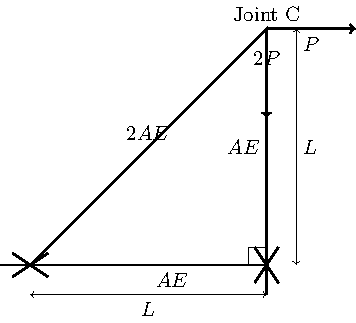
\includegraphics[width=0.7\linewidth]{figure/fig2/fig2.pdf}
		\caption{}
        \label{stemplot}

\end{figure}





 Given that $E = 2 * 10^{11} N/m^{2},A=10 mm^{2},L=1 m$ and $p=1 kN$.The horizontal displacement of joint C $\brak{in mm,up to one decimal place}$ is\\

 \item The water level in the the adjacent river is at an elevation of $+20.0 m$.Unit weight is $10 kN/m^{3}$.The factor of safety $\brak{up to two decimal places}$ against sand boiling for the proposed excavation is \\
\item A conventional drained triaxial compression test was conducted  on a normally consolidates clay sample under an effective pressure of $200 kPa$.the deviator stress at failure was found to be $400 kPa$. An identical specimen of the same clay sample is isotropically consolidated to a confining pressure of $200 kPa$ and subjected to standard undrained triaxial compression test. If the deviator stress at failure is $150 kPa$, the pore pressure developed $\brak{in kPa, up to one decimal place} $ is.\\
\item The void ratio of a soil is $0.55$ at an effective normal stress of $140 kPa$.The compression index of the soil is $0.25$.In order to reduce the void ratio to $0.4$, an increase in the magnitude of effective normal stress $\brak{in kPa,up to one decimal place}$ should be.\\
\item A rigid smooth retaining wall of height $7 m$ with vertical backface retains saturated day as backfil. the saturated unit weight and undrained cohesion of the backfill are $17.2 kN/m^{3}$ and $20 kPa$, respectively.The difference in the active lateral forces on the wall $\brak{in kN per meter lenght of wall,up to rwo decimal place}$,before and after the occurrence of tension crack is.\\
\item Rainfall depth over a watershed is monitored through six number of well distributed rain gauges. Gauges date are given below\\

\begin{table}[h!]
\centering
\begin{tabular}{|c|c|c|c|c|c|c|}
\hline
\textbf{Rain Gauge Number} & 1 & 2 & 3 & 4 & 5 & 6 \\
\hline
\textbf{Rainfall Depth (mm)} & 470 & 465 & 435 & 525 & 480 & 510 \\
\hline
\textbf{Area of Thiessen Polygon ($\times 10^4$ m$^2$)} & 95 & 100 & 98 & 80 & 85 & 92 \\
\hline
\end{tabular}
\end{table}
The Thiessen mean value $\brak{in mm, uo to one decimal place}$ of the rainfall is\\
\item The infiltration rate $f$ in a basin under ponding condition is given by $f=30+10e^{-2t}$,
where, $f$ is in mm/h and $t$ is time in hour. The depth of infiltration $\brak{in mm, up to one decimal place}$ during the last $20$ minute of a storm of $30$ minute duration is\\
\item In a laboratory, a flow experiment is performed over a hydraulic structure.The measured value of discharge and velocity are  $0.05 m^{3}/s$, and $0.25 m/s$, respectively.If the full scale structure $\brak{30 times bigger}$ is subjected to a discharge of $270 m^{3}/s$ then the time scale $\brak{mode to full scale}$ value $\brak{up to two decimal places}$ is\\
\item A water sample analysis data is given below\\
\begin{table}[h!]
    \centering
    \begin{tabular}{|c|c|c|}
        \hline
        \textbf{Ion} & \textbf{Concentration, mg/L} & \textbf{Atomic Weight} \\
        \hline
        $\text{Ca}^{2+}$ & 60 & 40 \\
        \hline
        $\text{Mg}^{2+}$ & 30 & 24.31 \\
        \hline
        $\text{HCO}_{3}^{-}$ & 400 & 61 \\
        \hline
    \end{tabular}
\end{table}
The carbonate hardness $\brak{expressed as mg/L of CaCO_{3}, up to one decimal place}$ for the water sample is\\
\item ultimate BOD $\brak{L_{0}}$ of a wastewater sample is estimated as $87\%$ of COD. The COD of this wastewater is $300 mg/L$. considering first order BOD reaction rate constant $k \brak{in mg/L, up to one decimal place}$ after three days of incubation at $27\%$ for this wastewater will be.









 
 \end{enumerate}





\end{document}
